%%%%%%%%%%%%%%%%%%%%%%%%%%%%%%%%%%%%%%%%%%%%%%%%%%%%%%%%%%%%%%%%%%%%%%
%%%%%%%%%%%%%%%%%%%%%%%%%%%%%%%%%%%%%%%%%%%%%%%%%%%%%%%%%%%%%%%%%%%%%%
\section{An energy estimate for doubly radial and odd minimizers}
\label{Sec:EnergyEstimate}

In this section we present a sharp estimate for the energy in $B_S$ of minimizers in the space $\widetilde{\H}^K_{0, \mathrm{odd}}(B_R)$ of the energy in $B_R$.



\todo[inline]{Rellenar}

In order to prove this result, we follow the ideas of Savin and Valdinocci in \cite{SavinValdinoci-EnergyEstimate}, where they establish the same estimate but for minimizers without any symmetry. The strategy is to compare $u$ with a suitable competitor which is constructed combining $u$ with an auxiliary function. In our case, since $u$ is a minimizer among functions in $\widetilde{\H}^K_{0, \mathrm{odd}}(B_R)$, we need to adapt the auxiliary function used in \cite{SavinValdinoci-EnergyEstimate} so that the resulting competitor is admissible, i.e., is a doubly radial function which is odd with  respect to the Simons cone $\ccal$.

The auxiliary function needed to build the competitor is defined as follows. For points $x\in \ocal$, we set
$$ \Psi_S(x) := \max\left\{-1+2\min\{(|x|-S-1)_+,1\},-\dist(x,\ccal) \right\},  $$
and we define it in $\ical$ by considering its odd reflection. In our arguments we will also use the following function and set:
$$ d_S(x) := \max\left\{1,\min\{S+1-|x|,\dist(x,\ccal)\} \right\},  $$
and
\begin{equation}
\label{Eq:DefOmegaS}
\Omega_S := \left( B_{S+2}\setminus \overline{B_s} \right) \cup \left( B_{S+2} \cap \{\dist(x,\ccal)< 1\}\right).
\end{equation} 

\begin{figure}
	\centering
	\begin{subfigure}{0.49\textwidth}
		\centering
		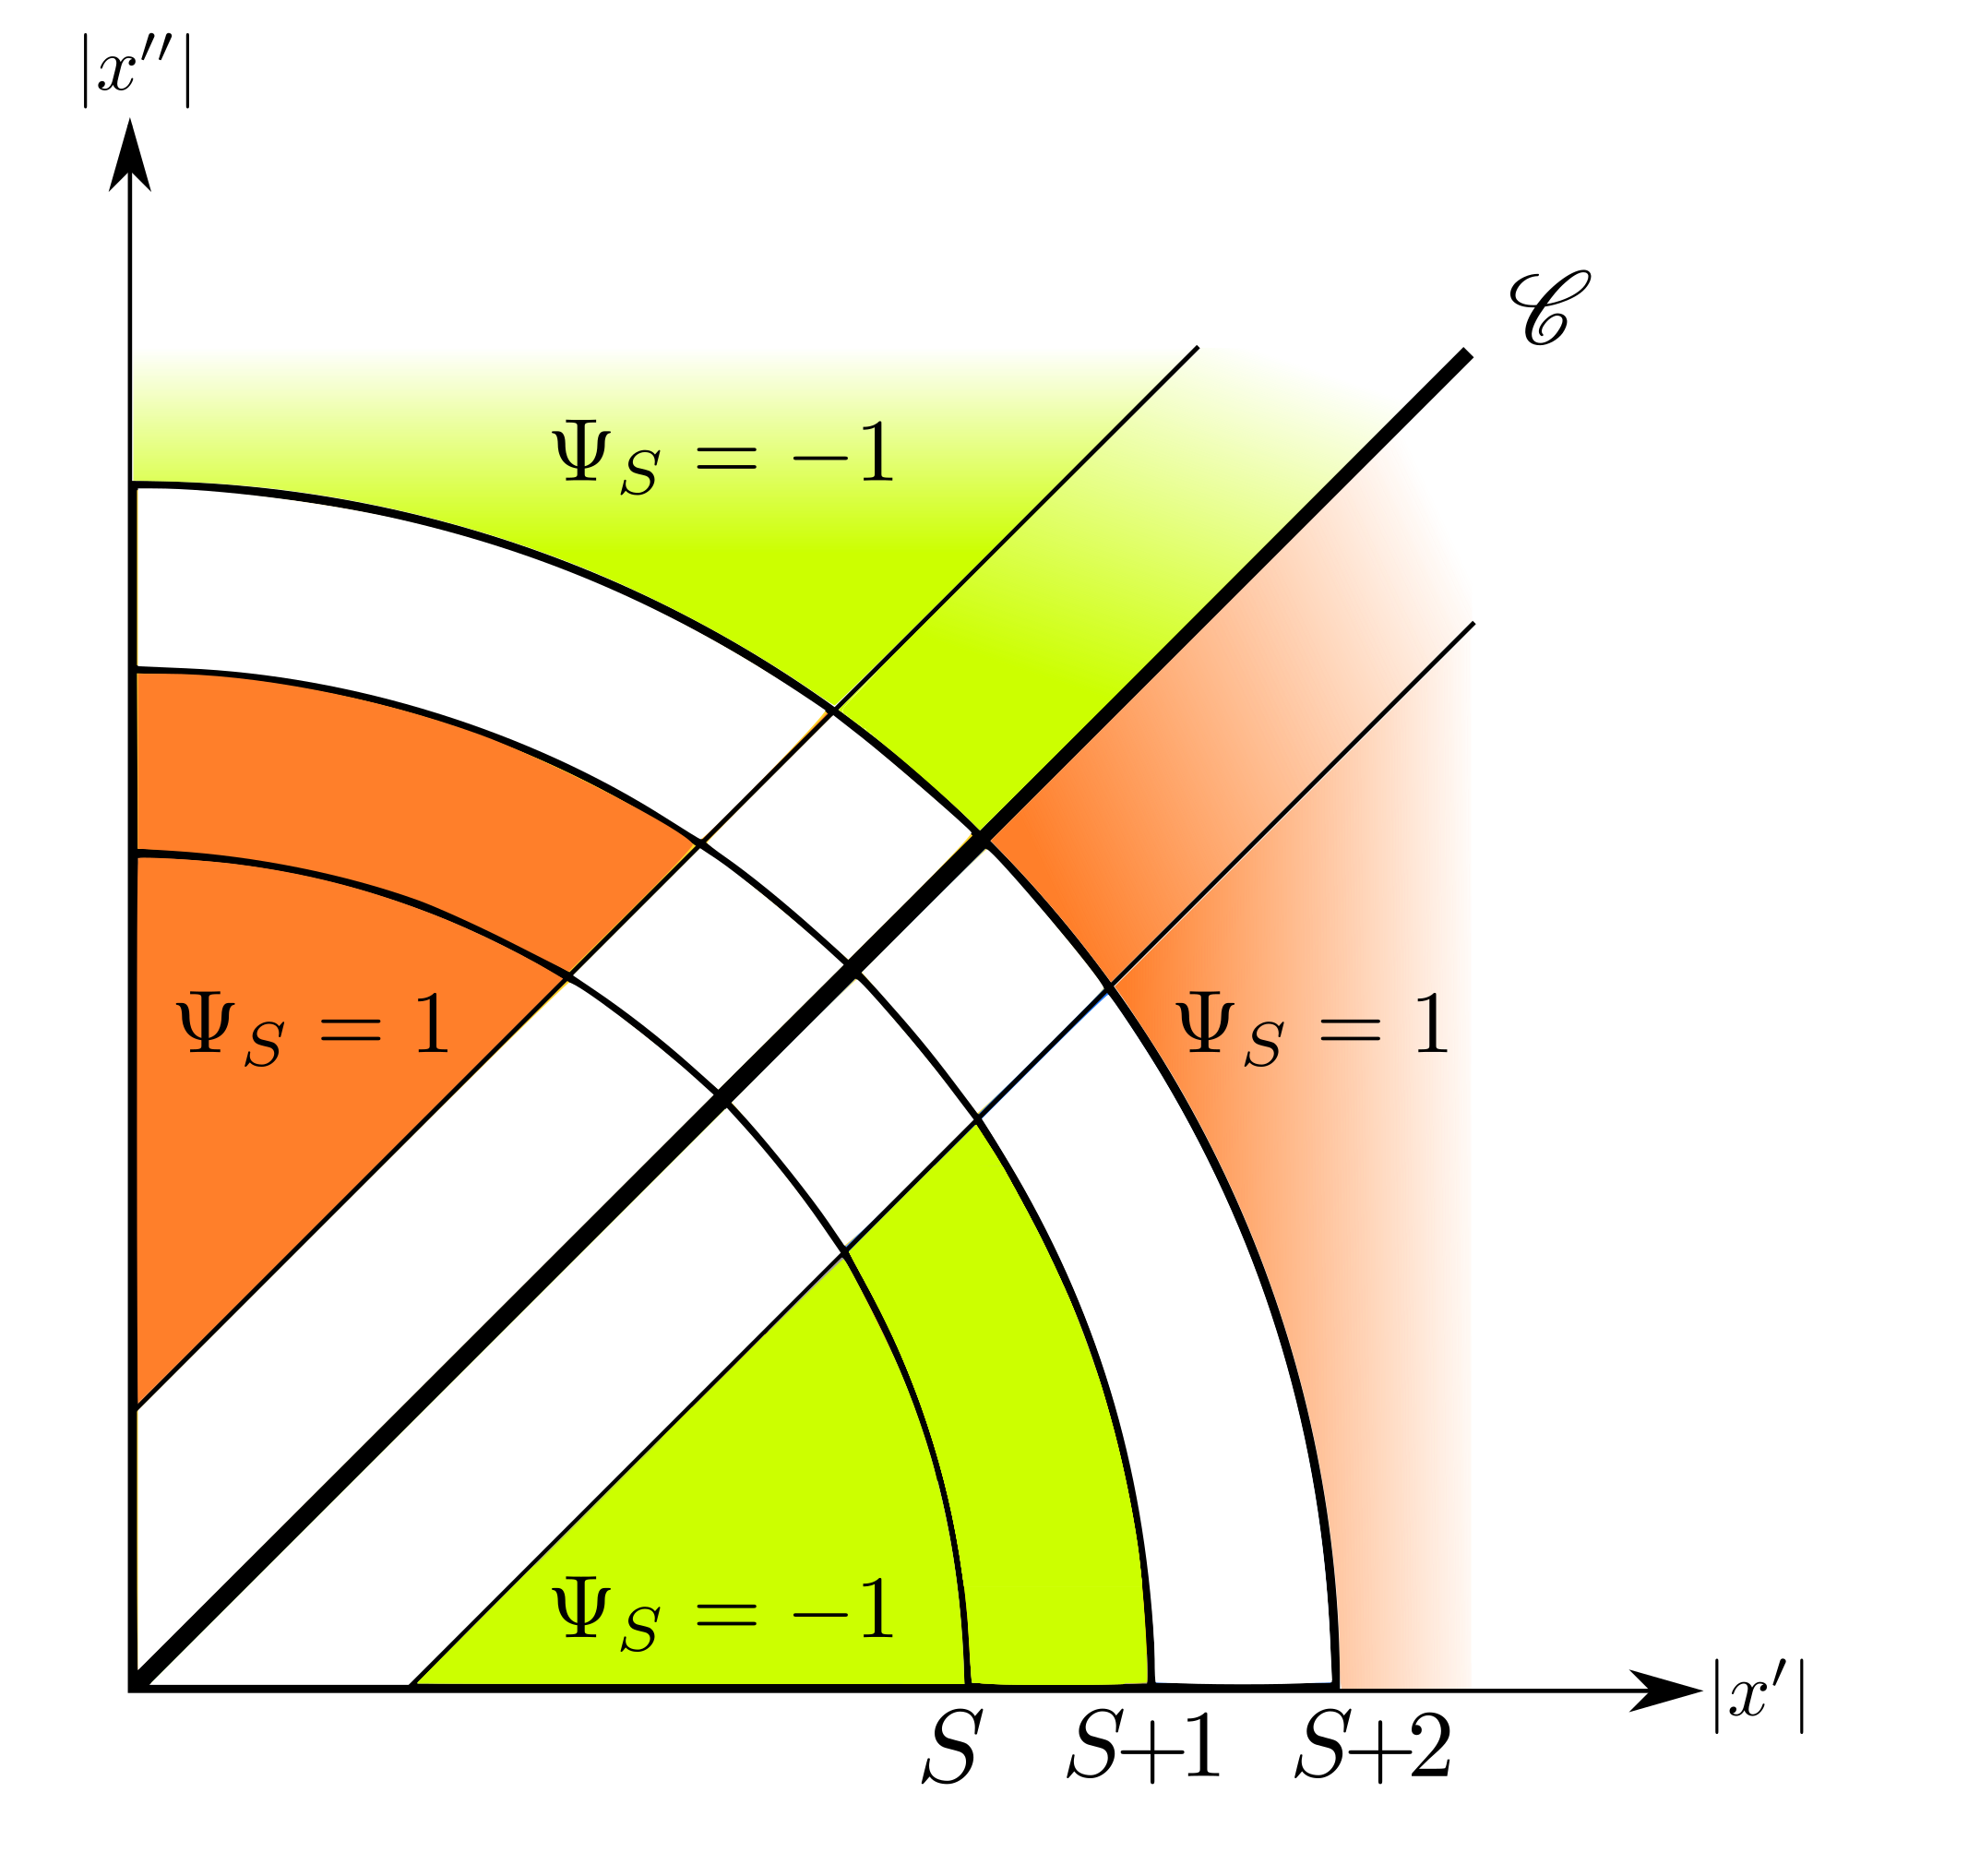
\includegraphics[width = \textwidth]{EnergyEstimatePsiS.png}
	\end{subfigure}
	\begin{subfigure}{0.49\textwidth}
		\centering
		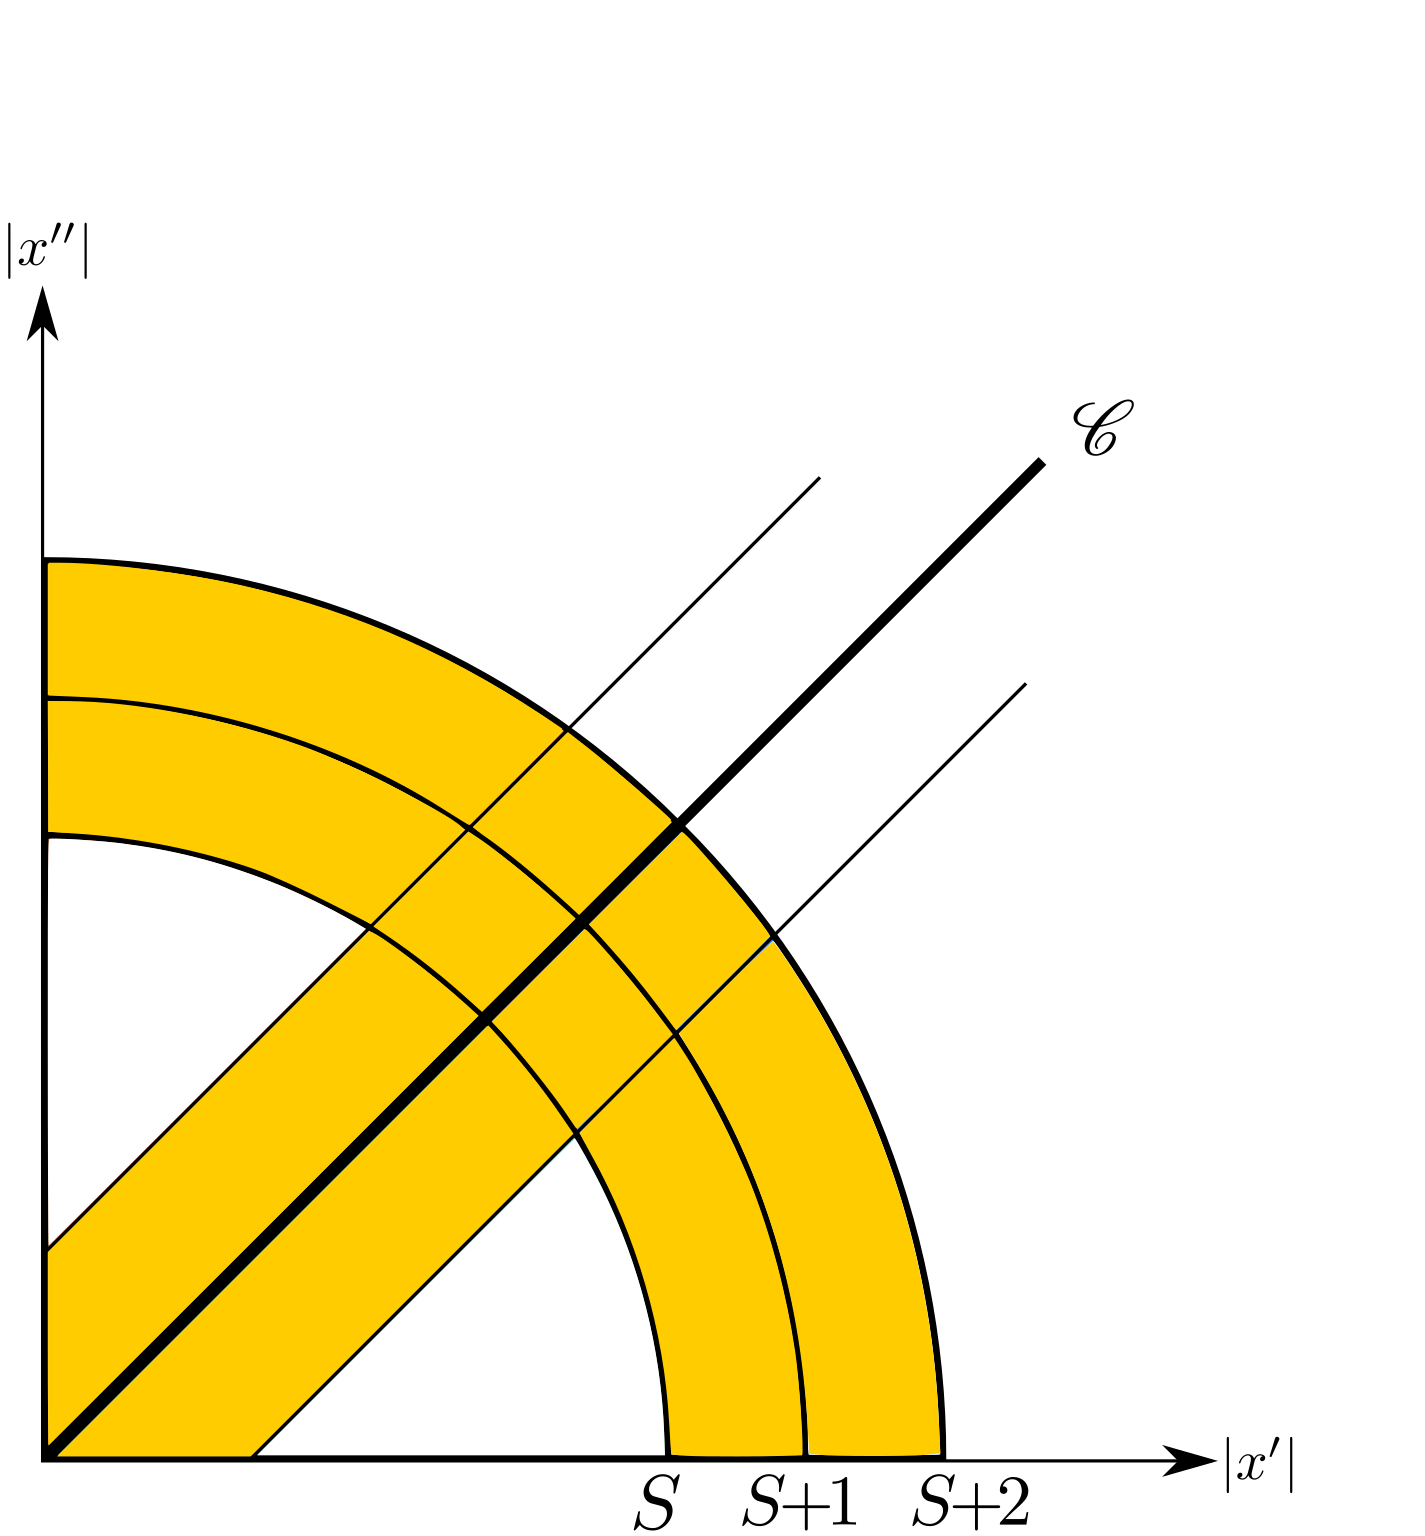
\includegraphics[width = \textwidth]{EnergyEstimateOmegaS.png}
	\end{subfigure}
	\caption{(a) The $1$ and $-1$ level sets of $\Psi_S$. (b) The set $\Omega_S$.}
	\label{Fig:PsiSandOmegaS}
\end{figure}

Note that both $\Psi_S$ and $d_S$ are Lipschitz functions, with Lipschitz norm independent of
$S$. Moreover $\Psi_S$ is odd and $d_S$ even with respect to the Simons cone. Regarding the set $\overline{\Omega_S}$, we can see it as the preimage of $1$ through $d_S$ inside $\overline{B_{S+2}}$.

Now we show some auxiliary results concerning the previous definitions.

\begin{lemma}
\label{Lemma: AdaptedLipschitzConditionWith_dFunction}
Given $S>0$, if either $(x,y) \in \left(\Omega_S\cap \ocal\right) \times \ical$ or $(x,y)\in \left(B_{S+2}\cap \ocal\right) \times \ocal$, then
$$ |\Psi_S(x) - \Psi_S(y)| \leq C \frac{|x-y|}{d_S(x)} \ \ \ \ \ \textrm{whenever} \ \ |x-y|\leq d_S(x), $$
with $C>0$ independent of $S$.
\end{lemma}

\begin{proof}
Note first that if $x\in \Omega_S \cap \ocal$, then $d_S(x)=1$ and the result is trivial by the Lipschitz continuity of $\Psi_S$. Hence, we only need to establish the result for the case $x\in B_S\cap \{\dist(x,\ccal)\geq 1\} \cap \ocal$ and $y\in \ocal$. Under these hypotheses, we have that $\Psi_S(x)=-1$ and $d_S(x) = \min\{S+1-|x|,\dist(x,\ccal)\}$. Moreover, since $x\in B_S$ and $\dist(x,\ccal)\geq 1$ we get $d_S(x) \leq S+1-|x|$. Therefore, if $|x-y|\leq d_S(x)$ we obtain
$$ |y|\leq |x-y| + |x| \leq d_S(x)+|x| \leq S+1. $$

Now we distinguish two cases, either $\{\dist(\cdot,\ccal)\geq 1\}$ or $\{\dist(\cdot,\ccal)\leq 1\}$. Assume first that $y\in B_{S+1} \cap \{\dist(\cdot,\ccal)\geq 1\}\cap \ocal$. Then, $\Psi_S(y)=-1$ and the result is trivial from being also $\Psi_S(x)=-1$. Thus, it only remains to show the result in the case $x\in B_S \cap \{\dist(\cdot,\ccal)\geq 1\}\cap \ocal$ and $y\in B_{S+1} \cap \{\dist(\cdot,\ccal)\leq 1\}\cap \ocal$. Note that under these assumptions, $\Psi_S(x)=-1$ and $\Psi_S(y)=-\dist(y,\ccal)$.


Given $x,y \in \R^{2m}$ it is easy to prove by using the triangular inequality and the definition of distance to the cone that
\begin{equation} \label{Eq:TriangularCone}
\dist(x,\ccal) \leq |x-y| + \dist(y,\ccal).
\end{equation}
Therefore we have
\begin{equation} \label{Eq:TriangularCone2}
1-|x-y|-\dist(y,\ccal) \leq 1-\dist(x,\ccal) \leq 0
\end{equation}
Now, multiplying \eqref{Eq:TriangularCone} by $|1-\dist(y,\ccal)|$ and using \eqref{Eq:TriangularCone2} we obtain
\begin{align*}
|1-\dist(y,\ccal)|\,\dist(x,\ccal) &\leq |1-\dist(y,\ccal)| \left(|x-y| + \dist(y,\ccal)\right) \\
%&= \left(1-\dist(y,\ccal)\right) \left(|x-y| + \dist(y,\ccal)\right) \\
&= |x-y|+\dist(y,\ccal) \left\{ -|x-y|+ 1- \dist(y,\ccal) \right\} \\
&\leq |x-y|.
\end{align*}

Hence,
$$ |\Psi_S(x)-\Psi_S(y)| = |1-\dist(y,\ccal)| \leq \frac{|x-y|}{\dist(x,\ccal)} \leq  \frac{|x-y|}{d_S(x)},$$
completing the proof.
\end{proof}

Another auxiliary result that we will need in the proof of Theorem~\ref{Th:EnergyEstimate} is the following estimate for the function $d_S$. 

\begin{lemma}
\label{Lemma:Integrability_dFunction}
Given $S>0$ we have
$$ \int_{B_{S+2}} d_S(x)^{-2\s} \d x \leq \begin{cases}
C \ S^{2m-2\s}\ \ \ \ &\textrm{if } \ \ \s\in(0,1/2),\\
C\ \log(S)\,S^{2m-2\s}\ \ \ \ &\textrm{if } \ \ \s=1/2,\\
C \ S^{2m-1}\ \ \ \ &\textrm{if } \ \ \s\in(1/2,1),\\
\end{cases} $$
with $C>0$ independent of $S$ and only depending on $m$ and $\s$.
\end{lemma}

\begin{proof}
In order to prove this result we first note that $d_S(x)=1$ in $\Omega_S$. Thus, the contribution to the integral of this part is just its measure, which is well known to be of order $2m-1$ (see the proof of the energy estimate in \cite{CabreTerraI}). That is,
$$\int_{\Omega_S} d_S(x)^{-2\s} \d x = |\Omega_S| \leq C\,S^{2m-1}.$$

For the other part of the integral we can write
\begin{align*}
\int_{B_{S+2}\setminus \Omega_S} d_S(x)^{-2\s} \d x &= \int_{B_{S}\cap \dist\{x,\ccal\}>1} d_S(x)^{-2\s} \d x \\
& \leq \int_{B_{S}\cap \dist\{x,\ccal\}>1} \left( S+1-|x| \right)^{-2\s} \d x + \int_{B_{S}\cap \dist\{x,\ccal\}>1} \dist(x,\ccal)^{-2\s} \d x.
\end{align*}
The desired estimate for the first integral can be found in \cite{SavinValdinoci-EnergyEstimate}. Therefore, in order to complete the proof it only remains to estimate the second integral. It can be estimated by writing it in $(y,z)$ variables, where
$$
y = \dfrac{|x'|+|x''|}{\sqrt{2}} \, \quad \text{ and } z = \dfrac{|x'|-|x''|}{\sqrt{2}}\,.
$$
In this case, $z$ is the signed distance to the cone. Thus,
\begin{align*}
\int_{B_{S}\cap \dist\{x,\ccal\}>1} \dist(x,\ccal)^{-2\s} \d x &\leq C \int \int_{B_{S}\cap \{y\geq|z|>1\}} |z|^{-2\s} \, (y^2-z^2)^{m-1} \d y\d z \\
& \leq C \int \int_{B_{S}\cap \{y\geq|z|>1\}} |z|^{-2\s} \, y^{2m-2} \d y\d z \\
& \leq C\, \int_1^S \d z \int_0^S \d y\ z^{-2\s} \, y^{2m-2} \\
& \leq C\, \left(\int_1^S z^{-2\s} \d z \right)  \left(  \int_0^S \d y \, y^{2m-2} \right) \\
& \leq \begin{cases}
C \ S^{2m-2\s}\ \ \ \ &\textrm{if } \ \ \s\in(0,1/2),\\
C\ \log(S)\,S^{2m-2\s}\ \ \ \ &\textrm{if } \ \ \s=1/2,\\
C \ S^{2m-1}\ \ \ \ &\textrm{if } \ \ \s\in(1/2,1).\\
\end{cases}
\end{align*}
\end{proof}


The last auxiliary result we need in order to establish the energy estimate is the following inequality.

\begin{lemma}
\label{Lemma: InteractionInequalityMinimumFunction}
Let $A\subset B_R \subset \R^{2m}$ be a set of double revolution such that $A^\star = A$ and let $\omega, \phi, \varphi \in \widetilde{\H}^K(B_R)$ be such that
$$\begin{cases}
\omega = \phi \leq \varphi \ \ \ \ \textrm{in } \ \ \ \ocal \setminus A\,,\\
\omega = \varphi \leq \phi \ \ \ \ \textrm{in } \ \ \ \ocal \cap A\,.
\end{cases}$$
Then, if $K$ satisfies \eqref{Eq:KernelInequalityReflexion}, it holds
\begin{align*}
I_\omega(\ocal\cap A, \ocal \setminus A) \leq I_\phi(\ocal\cap A, \ocal \setminus A) + I_\varphi(\ocal\cap A, \ocal \setminus A)\,,
\end{align*}
where $I_w(\cdot, \cdot)$ is the interaction defined in \eqref{Eq:DefIw}.
\end{lemma}

\begin{proof}
A simple computation shows that if $x\in \ocal \cap A$ and $y\in \ocal \setminus A$ we have that
$$ |\phi(x)-\phi(y)|^2+|\varphi(x)-\varphi(y)|^2\geq |\omega(x)-\omega(y)|^2. $$
Indeed,
\begin{align*}
|\phi(x)-\phi(y)|^2+|\varphi(x)&-\varphi(y)|^2 - |\omega(x)-\omega(y)|^2 \\
&= |\phi(x)-\phi(y)|^2+|\varphi(x)-\varphi(y)|^2 - |\varphi(x)-\phi(y)|^2 \\
&= \phi^2(x)-2\phi(x)\phi(y)+\varphi^2(y)-2\varphi(x)\varphi(y)+2\varphi(x)\phi(y) \\
&= \left( \phi(x) - \varphi(y)\right) ^2+2\left( \phi(x)-\varphi(x) \right) \left( \varphi(y)-\phi(y) \right) \\
&\geq 0.
\end{align*}
Therefore, by using this inequality and the reflexion property of the kernel, \eqref{Eq:KernelInequalityReflexion}, we obtain
\begin{align*}
I_\phi(\ocal\cap A, \ocal \setminus A) &+ I_\varphi(\ocal\cap A, \ocal \setminus A) - I_\omega(\ocal\cap A, \ocal \setminus A) = \\
&\hspace{-26mm}= \int_{\ocal\cap A} \d x \int_{\ocal\setminus A} \d y \left\{|\phi(x)-\phi(y)|^2+|\varphi(x)-\varphi(y)|^2-|\omega(x)-\omega(y)|^2 \right\} \left\{\overline{K}(x,y)-\overline{K}(x,y^\star)\right\} \\
&\hspace{-20mm}+ 2 \int_{\ocal\cap A} \d x \int_{\ocal\setminus A} \d y \left\{\phi^2(x)+\phi^2(y)+\varphi^2(x)+\varphi^2(y)-\omega^2(x)-\omega^2(y) \right\} \overline{K}(x,y^\star) \\
&\hspace{-26mm}\geq 2\int_{\ocal\cap A} \d x \int_{\ocal\setminus A} \d y \left\{
\phi^2(x)+\varphi^2(y)\right\} \overline{K}(x,y^\star) \geq 0.
\end{align*}
\end{proof}



With all these ingredients we can establish now the sharp energy estimate.

\begin{proof}[Proof of Theorem~\ref{Th:EnergyEstimate}]

Note that, by Lemma~\ref{Lemma:DecreaseEnergy}  we can assume without loss of generality that if $u$ is a minimizer of $\ecal$ in $B_R$, then $-1 \leq u \leq 1$, $u \geq 0$ in $\ocal$, and $u \leq 0$ in $\ical$. 

\textbf{Step 1. We show that $0\leq u < 1$ in $\ocal$.} 

In order to prove it we first need to show that $u$ is a weak solution of
\begin{equation}
\label{Eq:ProofEnergyEstimateProblemBR}
	\beqc{\PDEsystem}
	L_K  u &=& f(u) & \textrm{ in } B_R\,,\\
	u &=& 0 & \textrm{ in }\R^{2m} \setminus B_R.
	\eeqc
\end{equation}
To see this, we consider on the one hand perturbations $u +  \varepsilon \xi$, with $\xi \in \widetilde{\H}^K_{0, \,\mathrm{odd}}(B_R)$ and such that $\xi$ has compact support in $B_R$. Then, since $u$ is a minimizer among functions in $\widetilde{\H}^K_{0, \,\mathrm{odd}}(B_R)$, we get
$$
0 = \dfrac{\d}{\d \varepsilon}\evalat{\varepsilon = 0} \ecal(u +  \varepsilon \xi, B_R) = \langle u,\xi \rangle_{\widetilde{\H}^K_0(B_R)} - \langle f(u),\xi \rangle_{L^2(B_R)}\,.
$$
On the other hand, take $\xi \in \widetilde{\H}^K_{0, \,\mathrm{even}}(B_R)$. Since $u$ is odd with
respect to the Simons cone, so is $f(u)$. Then, by Remark~\ref{Remark:DecompositionHK} and the same
decomposition in $L^2(B_R)$, we find that
$$
\langle v_R,\xi \rangle_{\widetilde{\H}^K_0(B_R)} = 0 \quad \textrm{ and } \quad  \langle f(v_R),\xi \rangle_{L^2(B_R)} = 0\,.
$$
Therefore, we have that
$$
\langle u,\xi \rangle_{\widetilde{\H}^K_0(B_R)} = \langle f(u),\xi \rangle_{L^2(B_R)}
$$
for every $\xi \in\widetilde{\H}^K_0(B_R)$ with compact support in  $B_R$. Thus,
$$
\int_{\R^{2m}}\int_{\R^{2m}} \{u(x)-u(y)\}\{\xi(x)-\xi(y)\} K(|x-y|) \d x \d y = \int_{\R^{2m}} f(u(x)) \xi(x) \d x
$$
for every $\xi \in C^\infty_0(\Omega)$ that is double radially symmetric. 

By Proposition~\ref{Prop:WeakSolutionForAllTestFunctions}, $u$ is a weak solution of \eqref{Eq:ProofEnergyEstimateProblemBR}, and in view of the regularity theory for operators in $\lcal_0$ (see Remark~\ref{Remark:InteriorRegularity}), since $u$ is bounded, it is a classical solution.

From being $u$ a classical solution it is easy to show that it cannot be $1$ or $-1$ and therefore that it satisfies $0\leq u < 1$ in $\ocal$. That is, let us suppose that there exists $x_0\in\R^{2m}$ such that $|u(x_0)|=1$. Without loss of generality we can assume that $x_0\in\ocal\cap B_R$. Then, from equation \eqref{Eq:ProofEnergyEstimateProblemBR} and the fact of being $x_0$ an absolute maximum, we can arrive at a contradiction:
\begin{align*}
0 &= f(1) = f(u(x_0)) = L_K u(x_0) = \int_\ocal (1-u(y)) \overline{K}(x,y) + (1+u(y)) \overline{K}(x,y^\star)  \d y \\
&\geq \int_\ocal (1-u(y)) \overline{K}(x,y^\star) + (1+u(y)) \overline{K}(x,y^\star)  \d y = 2\int_\ocal \overline{K}(x,y^\star) \d y\\
&>0.
\end{align*}

\textbf{Step 2. We build a suitable competitor for $u$ and compare their energies.}

Now, for $x\in \ocal$ we define
$$ 
v(x) := \min\{u(x),\Psi_S(x)\}, 
$$
and we define it in $\ical$ by considering its odd reflection with respect to the Simons cone. Let us also define
$$
A = \{v=\Psi_S\} = \{\Psi_S \leq u\}. 
$$
Then, it is easy to check that we have the inclusions
\begin{equation}
\label{Eq:EnergyEstimateProofInclusionsA}
	B_{S+1} \subset A \subset B_{S+2}\,.
\end{equation}
To do it, note first that we only need to prove it inside $\ocal$, by the symmetry of $A$ with respect to the Simons cone. On the one hand, if $ x\in B_{S+1}\cap \ocal$, then $\Psi_S(x) = \max\{-1,-\dist(x,\ccal)\} \leq 0 \leq u(x)$, which yields $v(x) = \Psi_S(x)$ Thus, $x\in A\cap \ocal$. On the other hand, if $ x\in A\cap \ocal$ then $\Psi_S(x) \leq u(x) < 1$. This can only happen if $x\in B_{S+2}$.

Note that both $u$ and $v$ are equal outside $B_{S+2} \subset B_R$, and therefore $v$ is an admissible competitor. By comparing the energies of $u$ and $v$ we will obtain the desired estimate. 

Let us decompose the energy of $u$ in $B_R$ in terms of interactions between sets that involve $A$. That is,
\begin{align*}
\ecal(u,B_R) &= \frac{1}{2}I_u(\ocal \cap A, \ocal \cap A) + I_u(\ocal \cap A, \ocal \setminus A) \\
& \hspace{5mm} + \frac{1}{2}I_u\big((\ocal \setminus A) \cap B_R, (\ocal \setminus A) \cap B_R\big) + I_u\big((\ocal \setminus A) \cap B_R, \ocal \setminus B_R\big) \\
& \hspace{5mm} + \int_A G(u) + \int_{B_R\setminus A} G(u)
\end{align*}
Since $u$ is a minimizer, $v=\Psi_S$ in $A$ and $u=v$ outside of $A$,  from the previous expression we obtain
\begin{align*}
0 &\leq \ecal(v,B_R)-\ecal(u,B_R) = \frac{1}{2}I_{\Psi_S}(\ocal \cap A, \ocal \cap A) - \frac{1}{2}I_u(\ocal \cap A, \ocal \cap A)\\
& \hspace{5mm} + I_v(\ocal \cap A, \ocal \setminus A) - I_u(\ocal \cap A, \ocal \setminus A) + \int_A G(\Psi_S) - \int_{A} G(u)
\end{align*}
Since $v = \min\{u,\Psi_S\}$ in $\ocal$ we can apply Lemma \ref{Lemma: InteractionInequalityMinimumFunction} with $\omega = v$, $\Psi_S = \varphi$, and $u= \phi$, to get
\begin{align*}
\frac{1}{2}I_u(\ocal \cap A, \ocal \cap A) + \int_{A} G(u) &\leq \frac{1}{2}I_{\Psi_S}(\ocal \cap A, \ocal \cap A) + I_{\Psi_S}(\ocal \cap A, \ocal \setminus A) + \int_A G(\Psi_S)  \\
&= \ecal(\Psi_S, A) \leq \ecal(\Psi_S,B_{S+2})
\end{align*}
From this and using \eqref{Eq:EnergyEstimateProofInclusionsA}, we deduce an estimate for the energy of $u$ in $B_S$ as follows.
\begin{align*}
\ecal(u,B_S) &\leq \frac{1}{2}I_u(\ocal \cap A, \ocal \cap A) + \int_{A} G(u) + I_u(\ocal \setminus B_{S+1}, \ocal \cap B_S) \\
& \leq  \ecal(\Psi_S,B_{S+2}) + I_u(\ocal \setminus B_{S+1}, \ocal \cap B_S).
\end{align*}
Thus, to obtain the desired energy estimate we only have to bound the right-hand side of the last inequality.


\textbf{Step 3. We estimate the remaining terms.}

In the following arguments, we use the definition of the energy that involves the original kernel $K$ and not $\overline{K}$.

\textbf{3.1. Estimate for $\ecal(\Psi_S,B_{S+2})$.}
First, by using the change of variables given by $(\cdot)^\star$ and the ellipticity of $K$, \eqref{Eq:Ellipticity}, we obtain
\begin{align*}
\ecal(\Psi_S,B_{S+2}) &= \frac{1}{4} \int_{B_{S+2}} \int_{B_{S+2}} |\Psi_S(x)-\Psi(y)|^2K(|x-y|) \d x\d y \\
&\hspace{5mm} +\frac{1}{2} \int_{B_{S+2}} \int_{\R^{2m} \setminus B_{S+2}} |\Psi_S(x)-\Psi(y)|^2K(|x-y|) \d x\d y + \int_{B_{S+2}} G(\Psi_S) \\
&\leq \frac{1}{2} \int_{B_{S+2}} \int_{\R^{2m}} |\Psi_S(x)-\Psi(y)|^2K(|x-y|) \d x\d y + \int_{B_{S+2}} G(\Psi_S) \\
&= \int_{B_{S+2} \cap \ocal} \int_{\R^{2m}} |\Psi_S(x)-\Psi(y)|^2K(|x-y|) \d x\d y + \int_{B_{S+2}} G(\Psi_S) \\
&= \Lambda \int_{B_{S+2} \cap \ocal} \int_{\R^{2m}} \frac{|\Psi_S(x)-\Psi(y)|^2}{|x-y|^{n+2\s}} \d x\d y + \int_{B_{S+2}} G(\Psi_S).
\end{align*}
Now, we split the domain of integration of the kinetic energy into three parts.
\begin{align*}
\ecal(\Psi_S,B_{S+2}) &\leq \Lambda \int_{B_{S+2} \cap \ocal} \int_{\ocal} \frac{|\Psi_S(x)-\Psi(y)|^2}{|x-y|^{n+2\s}} \d x\d y \\
&\hspace{5mm} + \Lambda \int_{\Omega_S \cap \ocal} \int_{\ical} \frac{|\Psi_S(x)-\Psi(y)|^2}{|x-y|^{n+2\s}} \d x\d y \\
&\hspace{5mm} + \Lambda \int_{(B_{S+2}\setminus \Omega_S) \cap \ocal} \int_{\ical} \frac{|\Psi_S(x)-\Psi(y)|^2}{|x-y|^{n+2\s}} \d x\d y + \int_{B_{S+2}} G(\Psi_S) \\
&=:I_1+I_2+I_3+I_G,
\end{align*}
where $\Omega_S$ is defined in \eqref{Eq:DefOmegaS}. 

Let us estimate this four integrals. 
\begin{align*}
I_1 &= \Lambda \int_{B_{S+2} \cap \ocal} \int_{\ocal} \frac{|\Psi_S(x)-\Psi(y)|^2}{|x-y|^{n+2\s}} \d x\d y\\
&= \Lambda \int_{B_{S+2} \cap \ocal} \int_{\ocal\cap\{|x-y|\leq d_S(x)\}} \frac{|\Psi_S(x)-\Psi(y)|^2}{|x-y|^{n+2\s}} \d x\d y\\
&\hspace{5mm} + \Lambda \int_{B_{S+2} \cap \ocal} \int_{\ocal\cap\{|x-y|\geq d_S(x)\}} \frac{|\Psi_S(x)-\Psi(y)|^2}{|x-y|^{n+2\s}} \d x\d y\\
&\leq C \int_{B_{S+2} \cap \ocal} d_S(x)^{-2}\int_{\ocal\cap\{|x-y|\leq d_S(x)\}} |x-y|^{2-n-2\s} \d y\d x\\
&\hspace{5mm} + C \int_{B_{S+2} \cap \ocal} \int_{\ocal\cap\{|x-y|\geq d_S(x)\}} |x-y|^{-n-2\s} \d x\d y\\
&\leq C \int_{B_{S+2} \cap \ocal} d_S(x)^{-2}\int_0^{d_S(x)} \rho^{1-2\s} \d \rho\d x + C \int_{B_{S+2} \cap \ocal}  \int_{d_S(x)}^\infty \rho^{-1-2\s} \d\rho \d x\\
&\leq C \int_{B_{S+2} \cap \ocal} d_S(x)^{-2\s} \d x,
\end{align*}
where in the first inequality we have used Lemma~\ref{Lemma: AdaptedLipschitzConditionWith_dFunction} and the uniform bound of $\Psi_S$. The bound of $I_2$ is essentially the same using also Lemma~\ref{Lemma: AdaptedLipschitzConditionWith_dFunction} and the inclusion $\Omega_S \subset B_{S+2}$. That is,
\begin{align*}
I_2 &= \Lambda \int_{\Omega_S \cap \ocal} \int_{\ical} \frac{|\Psi_S(x)-\Psi(y)|^2}{|x-y|^{n+2\s}} \d x\d y\\
&= \Lambda \int_{\Omega_S \cap \ocal} \int_{\ical\cap\{|x-y|\leq d_S(x)\}} \frac{|\Psi_S(x)-\Psi(y)|^2}{|x-y|^{n+2\s}} \d x\d y\\
&\hspace{5mm} + \Lambda \int_{\Omega_S \cap \ocal} \int_{\ical\cap\{|x-y|\geq d_S(x)\}} \frac{|\Psi_S(x)-\Psi(y)|^2}{|x-y|^{n+2\s}} \d x\d y\\
&\leq C \int_{\Omega_S \cap \ocal} d_S(x)^{-2}\int_0^{d_S(x)} \rho^{1-2\s} \d \rho\d x + C \int_{\Omega_S \cap \ocal}  \int_{d_S(x)}^\infty \rho^{-1-2\s} \d\rho \d x\\
&\leq C \int_{\Omega _S\cap \ocal} d_S(x)^{-2\s} \d x \leq C \int_{B_{S+2} \cap \ocal} d_S(x)^{-2\s} \d x.
\end{align*}
For the case of $I_3$, we use the fact that given $x\in (B_{S+2}\setminus \Omega_S)\cap \ocal$, then $\dist(x,\ccal)\geq d_S(x)$ and therefore $\ical \subset \R^{2m}\setminus B_{d_S(x)}(x)$.
\begin{align*}
I_3 &= \Lambda \int_{(B_{S+2}\setminus \Omega_S) \cap \ocal} \int_{\ical} \frac{|\Psi_S(x)-\Psi(y)|^2}{|x-y|^{n+2\s}} \d x\d y \leq C \int_{(B_{S+2}\setminus \Omega_S) \cap \ocal} \int_{\R^{2m}\setminus B_{d_S(x)}(x)} |x-y|^{-n-2\s} \\
&\leq C \int_{B_{S+2} \cap \ocal} \int_{d_S(x)}^\infty \rho^{-1-2\s} \d \rho\d x \leq C \int_{B_{S+2} \cap \ocal} d_S(x)^{-2\s} \d x.
\end{align*}
Finally, we estimate $I_G$. Since $\Psi_S$ is either $1$ or $-1$ in $B_{S+2}\setminus \Omega_S$, and $G(-1)=G(1)=0$, we have
\begin{align*}
I_G = \int_{B_{S+2}} G(\Psi_S) = \int_{\Omega_S} G(\Psi_S) \leq C | \Omega_S| \leq C\,S^{2m-1}\,.
\end{align*}
Therefore, we obtain
\begin{align*}
\ecal(\Psi_S,B_{S+2}) &\leq C \left(\int_{B_{S+2} \cap \ocal} d_S(x)^{-2\s} \d x + S^{2m-1} \right)\leq C\left(\int_{B_{S} \cap \ocal} d_S(x)^{-2\s} \d x + S^{2m-1} \right).
\end{align*}

%%%%%%%%%

\textbf{3.2. Estimate for $I_u(\ocal \setminus B_{S+1}, \ocal \cap B_S)$.} First, we claim that $|x-y|\geq d_S(x)$ whenever $x\in B_S\cap \ocal$ and $y\in \R^{2m}\setminus B_{S+1}$. Indeed, if $x\in B_S$, then $d_S(x) \leq S+1-|x|$ and therefore we have $|x-y|\geq |y|-|x|\geq |y|+d_S(x)-S-1 \geq  d_S(x)$, since $|y| \geq S+1$. Thus, using this and the ellipticity of $K$ we get
\begin{align*}
I_u(\ocal \setminus B_{S+1}, \ocal \cap B_S) &\leq C \int_{B_S \cap \ocal} \d x \int_{\R^{2m}\setminus B_{S+1}} \d y \ \frac{|u(x)-u(y)|^2}{|x-y|^{2m+2\s}} \\
& C \leq \int_{B_S \cap \ocal} \d x \int_{|x-y|\geq d_S(x)} \d y \ |x-y|^{-2m-2\s} \\
&\leq C \int_{B_S \cap \ocal} d_S(x)^{-2\s} \d x.
\end{align*}

\textbf{Step 4. Conclusion.}

Finally, by adding up the estimates of Step~3 and applying Lemma~\ref{Lemma:Integrability_dFunction}, we obtain the desired result. That is,
\begin{align*}
\ecal(u,B_S) &\leq \ecal(\Psi_S,B_{S+2}) + I_u(\ocal \setminus B_{S+1}, \ocal \cap B_S) \leq C\left(\int_{B_S \cap \ocal} d_S(x)^{-2\s} \d x + S^{2m-1} \right)\\
&\leq \begin{cases}
C \ S^{2m-2\s}\ \ \ &\textrm{if } \ \ \s\in(0,1/2),\\
C\ \log(S)\,S^{2m-2\s}\ \ \ \ &\textrm{if } \ \ \s=1/2,\\
C \ S^{2m-1}\ \ \ \ &\textrm{if } \ \ \s\in(1/2,1).\\
\end{cases}
\end{align*}
\end{proof}
